\section{Results}
\label{sec:results}

This section addresses the four questions in the order in which they were
posed. The results pertain to the $0.05\,\%$ ETH/USDC pool and cover thirteen
2024 windows that no policy observed during training. Where a learned policy is
involved, results are averaged across five seeds. Statistics are computed on
the exact backtester, and the testbed applies its frictions to whichever leg is
active.

\subsection{Where the fees fail}

A passive position collects fees and bears the cost of price movements it
cannot follow. Table~\ref{tab:decomposition} separates these two components.
Fee income declines as the band widens, while impermanent loss declines more
rapidly. The liquidity leg is negative across the passive ladder. The deficit
narrows as the band widens, but its sign does not change. Even the strongest
passive rule finishes below the buy-and-hold basket.

Narrowing the band increases fee income and also increases the magnitude of
impermanent loss. The two quantities grow in roughly equal proportion, so their
ratio remains approximately constant across the widths reported in
Table~\ref{tab:decomposition}. Concentration therefore leaves the shortfall
intact. It changes the variance of the outcome rather than its sign.

The window-level results are consistent with the aggregate pattern. The final
column of Table~\ref{tab:decomposition} counts negative liquidity windows by
rule. This count declines as the band widens but never reaches zero. Losses concentrate in windows where the price
trends or jumps. In range-bound windows the narrower bands change sign and fee
income covers the shortfall. Table~\ref{tab:regimes} reports the same pattern
by regime.

Active rebalancing does not remedy the arithmetic and in fact worsens it. The
two rebalancing rules in Table~\ref{tab:decomposition} collect more fee income
than any one-shot rule because they keep the band close to the price. They also
incur larger realised losses and execution costs. Both finish further behind
the basket than any passive rule. \textsf{tau\_reset} loses in all four
regimes.
\textsf{cost\_aware} earns only in bull windows. For this pool and year, fee
income does not cover the price risk a position carries. Frequent action adds
cost without changing the sign. The next subsection examines whether a learned
policy can exploit this structure.

The decisive cost is the one the position cannot avoid. Table~\ref{tab:friction}
removes one cost term at a time from the same ledger. When impermanent loss is
removed, the recentring rule reverses from a large loss to a large gain. The
one-shot band also gains materially. When gas and slippage are removed, the
one-shot band barely changes. The frequently rebalancing rule recovers its
execution costs but remains far behind. The one-shot rule loses to the basket
because of price travel rather than execution. The recentring rule adds
execution costs to a loss it has already increased.

A higher fee tier reverses the sign of the passive arithmetic.
Table~\ref{tab:contrast} and Fig.~\ref{fig:fee-tier} rerun the ladder on the
$0.30\,\%$ pool. The wide and full-range arms, together with both static
widths, finish ahead of the opening basket. A larger fee per unit of volume
covers the loss to informed flow. The two rebalancing rules still lose. The
contrast indicates what the primary pool would require. The same widths cross
from deficit to surplus on a tier with six times the fee per swap.

\begin{table}[tbp]
\caption{Friction ablation on the $0.05\,\%$ pool over the thirteen evaluation
windows. Values are mean PnL in USDC with Sharpe in parentheses. The one-shot
rule is \textsf{passive\_wide}; the recentring rule is \textsf{tau\_reset}.
\textsf{no IL} removes the impermanent-loss term. \textsf{no gas} and
\textsf{no slippage} remove their cost term. \textsf{flat gas} re-prices each
rebalance at a flat 30 gwei base fee plus a 3\,\% tip at \usdc{3000} per ETH.}
\label{tab:friction}
\centering
\small
\begin{tabular}{@{}L{0.28\linewidth}rr@{}}
\toprule
\textbf{Variant} & \textbf{one-shot wide} & \textbf{recentring} \\
\midrule
full & $+1\,623$ (1.53) & $-17\,680$ ($-5.81$) \\
no IL & $+5\,172$ (1.65) & $+31\,224$ (12.84) \\
no gas & $+1\,659$ (1.53) & $-8\,908$ ($-3.02$) \\
no slippage & $+1\,624$ (1.53) & $-12\,359$ ($-3.91$) \\
flat gas & $+1\,583$ (1.53) & $-18\,303$ ($-6.32$) \\
\bottomrule
\end{tabular}
\end{table}

\begin{table}[tbp]
\caption{The rule ladder on the $0.30\,\%$ (3000 pips) tier, mean over the
thirteen evaluation windows. Net is the liquidity leg's excess over the
opening basket. The two static rows are the price-equivalent of the primary
pool's $250$- and $1000$-spacing arms at this pool's spacing of $60$.}
\label{tab:contrast}
\centering
\small
\begin{tabular}{@{}L{0.38\linewidth}rrr@{}}
\toprule
\textbf{Rule} & \textbf{PnL} & \textbf{Sharpe} & \textbf{Net} \\
\midrule
\textsf{hodl} opening band & $+1\,361$ & 2.06 & $-109$ \\
\textsf{passive\_narrow} ($\pm5\,\%$) & $+1\,432$ & 2.89 & $-38$ \\
\textsf{passive\_wide} ($\pm20\,\%$) & $+1\,808$ & 3.33 & $+338$ \\
\textsf{full\_range\_v2} & $+2\,188$ & 1.30 & $+719$ \\
static width $42$ spacings & $+1\,893$ & 3.45 & $+423$ \\
static width $167$ spacings & $+2\,204$ & 1.97 & $+734$ \\
\textsf{tau\_reset} & $-20\,702$ & $-15.89$ & $-22\,172$ \\
\textsf{cost\_aware} & $-2\,101$ & $-0.27$ & $-3\,571$ \\
\bottomrule
\end{tabular}
\end{table}

\begin{figure}[tbp]
\centering
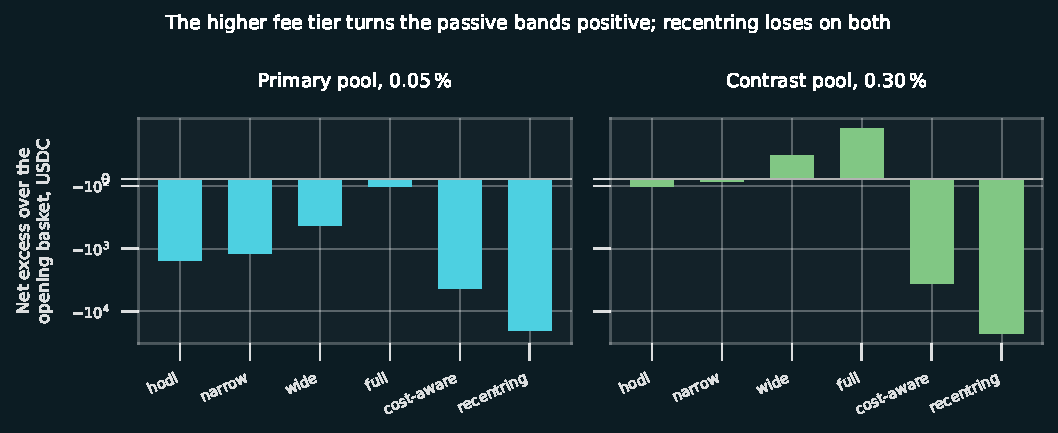
\includegraphics[width=\linewidth]{figures/fee_tier.pdf}
\caption{Net excess over the opening basket on the two fee tiers, mean over the
thirteen 2024 evaluation windows. The primary pool is the $0.05\,\%$ tier. The
contrast pool is the $0.30\,\%$ tier. Bars above zero beat the passive holding.
The vertical axis is symmetric-logarithmic so the recentring rules remain
visible.}
\label{fig:fee-tier}
\end{figure}

\begin{table}[tbp]
\caption{Fee income against impermanent loss on the thirteen evaluation
windows. Values are mean per window in USDC. Fees, impermanent loss, gas and
slippage are measured against the pure buy-and-hold basket. The liquidity net
therefore excludes the basket's own \usdc{2288}, and the hedge column is zero
for the unhedged rules. The last column counts windows in which the liquidity
net is negative.}
\label{tab:decomposition}
\centering
\small
\begin{tabular}{@{}L{0.17\linewidth}rrrrrr@{}}
\toprule
\textbf{Policy} & \textbf{Fees} & \textbf{IL} & \textbf{Costs} & \textbf{LP net} & \textbf{Hedge} & \textbf{Net<0} \\
\midrule
\textsf{hodl} & $+4\,734$ & $-6\,287$ & $0$ & $-1\,553$ & $0$ & 6/13 \\
\textsf{passive\_narrow} & $+4\,266$ & $-5\,435$ & $-37$ & $-1\,206$ & $0$ & 5/13 \\
\textsf{passive\_wide} & $+2\,921$ & $-3\,549$ & $-37$ & $-665$ & $0$ & 4/13 \\
\textsf{full\_range\_v2} & $+362$ & $-430$ & $-37$ & $-106$ & $0$ & 3/13 \\
\textsf{tau\_reset} & $+43\,029$ & $-48\,904$ & $-14\,093$ & $-19\,968$ & $0$ & 13/13 \\
\textsf{cost\_aware} & $+19\,833$ & $-22\,038$ & $-2\,075$ & $-4\,280$ & $0$ & 10/13 \\
\bottomrule
\end{tabular}
\end{table}

\subsection{Why the first policies failed}

The first question was whether the learner could act at all. On the original
interface it could not. The timing, centre and width decisions were encoded as
91 actions, and the reward was measured against a basket that moved whenever
the band was rebalanced. The trained policies churned. They shifted the band at
frequent intervals and paid gas and slippage whenever they moved. Reducing the grid to 28
actions changed the magnitude of the churn but not the behaviour. The collapse
was not an optimisation accident. The reward gradient was dominated by the
decision to act or hold, and the observation provided no signal about the
position of the price within the band.

The repairs were applied in sequence rather than as a factorial ablation. The
evidence therefore measures the cumulative effect of the sequence and not the
marginal effect of any single change. Three interface defects were corrected
first. The observation gained the distance to both band edges and the band
width. The reward was measured against the fixed opening basket rather than a
basket that moved on rebalance. Training windows were resampled from
2022--2023 rather than replayed from one fixed month. Two further defects
emerged during these repairs. Slippage was charged on the whole position value
rather than the inventory actually swapped, and fee credit was taken from
global fee growth rather than the position's exact share of the occupied
liquidity segments. Both were corrected before any result reported here.

Three changes to the learning setup followed. Stabilising the update targets
made the five seeds hold for the full episode with zero rebalances and turned
a strongly negative return into a mildly negative one. The update remained inside
its trust region. The policy had learned to do nothing, which tied
\textsf{hodl}. Reducing the action space to a one-shot band choice and
lengthening the effective horizon together gave the width decision a usable
signal. The first pilot that genuinely selected a band matched the full-range
rule's PnL with a higher Sharpe ratio and beat \textsf{hodl} on both PnL and
Sharpe.

The hedge head failed in its first joint run. The seeds held the liquidity
position for the full episode and collapsed the hedge ratio to a seed-specific
constant. The seed selected on the training curve lost out of sample. The
objective had never rewarded tail protection, and selection used the training
return rather than a validation statistic. The final training run added a
penalty on the conditional tail of joint equity and selected checkpoints by
validation Sharpe. That run produced the final policy evaluated below.

The regime label is an input rather than a target, but it still shapes what the
policy learns. A second arm trained five seeds with the regime feature frozen
to a constant. Its mean Sharpe is numerically higher, but the paired difference
is indistinguishable from zero at this sample size. Its mean CVaR is worse,
with an interval that excludes zero. The live regime feature therefore buys
tail protection rather than return. The ablated seeds diverge more widely. One
never deploys, and two widen to the $1000$-spacing band. The arm's best
validation seed finishes worst out of sample. The selection signal remains weak
even for a policy that learns. Appendix~\ref{app:ablations} reports the arm in
full.

\begin{figure}[tbp]
\centering
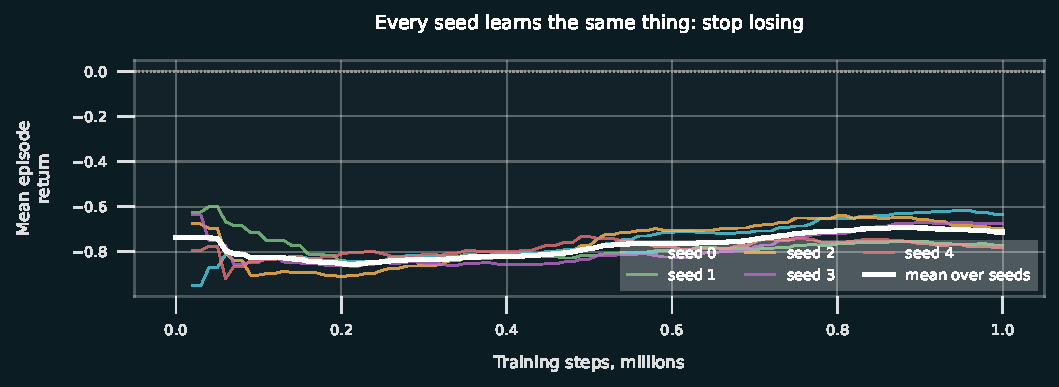
\includegraphics[width=\linewidth]{figures/learning_curves.pdf}
\caption{Training reward of the five seeds of the main joint run. The vertical
axis is mean episode return against timesteps. The return is measured against
the opening basket and normalised by capital. A less negative curve is a policy
that has learned to lose less.}
\label{fig:learning-curves}
\end{figure}

\subsection{Whether one policy does better}

The pre-registered comparison uses the strongest hand-written rules, the best
static width selected on the training split, and a hedged benchmark with a
matched delta. Table~\ref{tab:aggregate} reports the levels, and
Table~\ref{tab:paired} reports the paired per-window differences on which the
decision rule depends.

\begin{figure}[tbp]
\centering
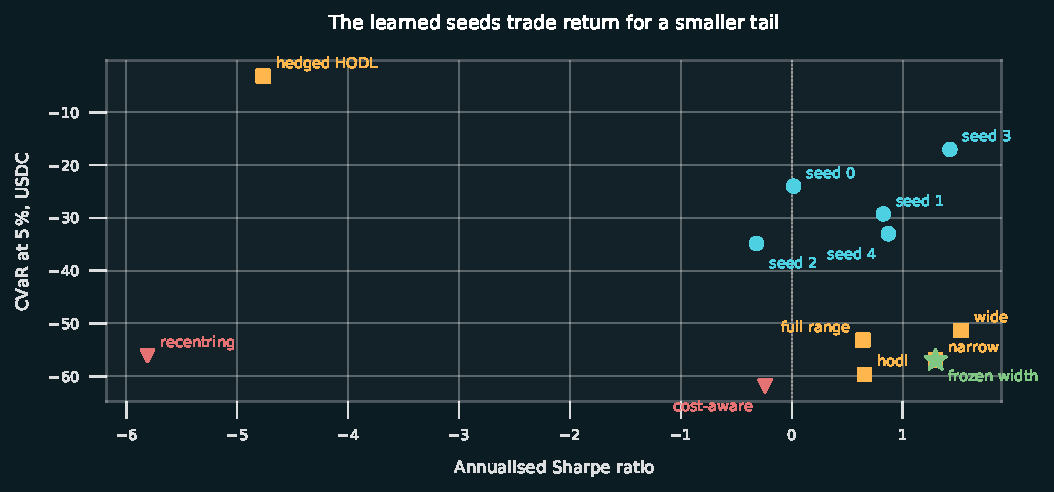
\includegraphics[width=\linewidth]{figures/risk_return.pdf}
\caption{Annualised Sharpe against CVaR at the $5\,\%$ level for the rules in
the evaluation ladder, mean over the thirteen 2024 windows. Up and to the right
is better. The star marks the static width frozen on the training split. The
learned seeds sit above the unhedged rules on the tail axis but left of the
best static width on the return axis.}
\label{fig:risk-return}
\end{figure}

The frozen comparator provides the first test. On the training split the
narrowest of the three width arms had the best Sharpe, so the protocol froze
that width. Appendix~\ref{app:ablations} lists the training and evaluation
scores. The learned mean loses to the frozen width on the evaluation windows.
The paired Sharpe difference is $-0.733$ with an interval of $[-1.355,-0.041]$
that excludes zero. The learned mean also loses to the wide band, with an
interval that excludes zero. The Sharpe clause of the pre-registered rule
fails.

The tail clause holds against the unhedged benchmarks.
Table~\ref{tab:aggregate} reports the levels, and Table~\ref{tab:paired} reports
the paired differences. The CVaR differences against unhedged benchmarks are
positive, with intervals that exclude zero. The clause fails against the
delta-matched hedge, whose paired interval excludes zero in the opposite
direction. Both clauses must hold for a positive verdict, so the pre-registered
rule yields none. The evidence supports a reduction in tail risk but not a
superior return.

Aggregation across seeds conceals the strongest individual policy. The seed
with the highest validation Sharpe during training deployed the $250$-spacing
band throughout the thirteen windows and held it. Its row in Table~\ref{tab:aggregate}
is the best seed. Its Sharpe is statistically indistinguishable from that of
the frozen width, while its CVaR is better with an interval that excludes zero.
It beats the delta-matched hedge on Sharpe and loses to it on CVaR. A single
seed is not the pre-registered unit, and a seed chosen after observing the
evaluation windows cannot support the verdict. This seed did have the best
validation Sharpe of the five on the training split, so its selection did not
use the evaluation year.

The seeds agree on timing but disagree on width and hedge. A seed deploys once
at the start of the episode and holds. Table~\ref{tab:actions} records one
rebalance per episode for the five seeds. Seed zero uses the narrow band. Three
seeds use the $250$-spacing band throughout the evaluation year. Seed one uses
the $250$-spacing band in twelve of the thirteen windows. Hedge ratios are partial and
differ by seed. The learned policy sets a band and a hedge ratio rather than a
timing rule. Its preferred width is the static band with the best Sharpe on the
evaluation windows, although that band was not the frozen comparator.
Figure~\ref{fig:action-map} shows deployment by seed.

\begin{figure}[tbp]
\centering
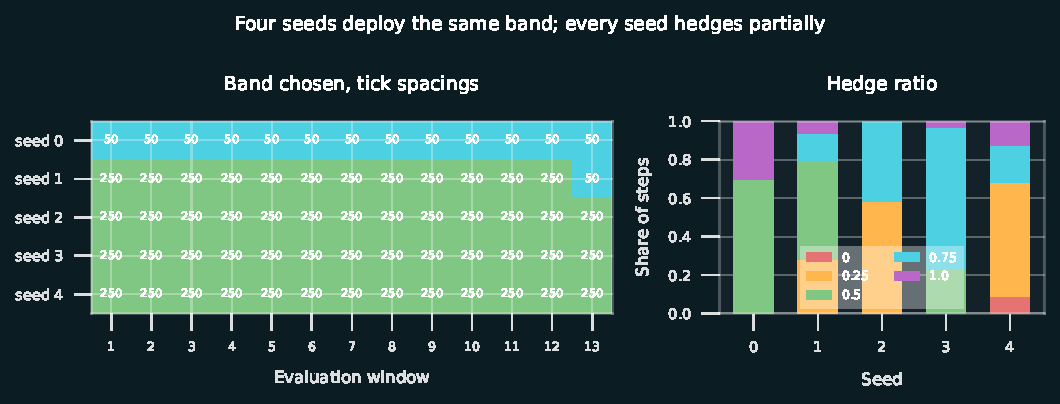
\includegraphics[width=\linewidth]{figures/action_map.pdf}
\caption{What the learned seeds chose on the thirteen evaluation windows. The
left panel shows the band half-width in tick spacings chosen at deployment,
with \textsf{hold} where the seed never deployed. The right panel shows the
share of decision steps spent at the five short ratios.}
\label{fig:action-map}
\end{figure}

The worst window for the one-shot rules and the learned mean is the single
high-volatility window. Table~\ref{tab:regimes} reports its PnL and tail loss by
regime. Raw PnL and tail risk rank the policies consistently across the year.
No paired PnL difference against the ladder excludes zero except the comparison
with \textsf{tau\_reset}, so the return evidence remains inconclusive at this
sample size.

\begin{table}[tbp]
\caption{Performance in the 2024 evaluation on the $0.05\,\%$ (500 pips)
ETH/USDC pool, mean over the thirteen windows of the 2024 tiling. PnL and
excess are USDC per episode. Excess is measured against the pure buy-and-hold
basket, the study's HODL numeraire. The row for the learned mean averages the
five seeds. The row for the best seed reports the seed with the highest
validation Sharpe on the training split. Rebalances counts executed moves per
episode. The frozen comparator selected on the training split is the half-width
of 50 tick spacings, the \textsf{passive\_narrow} row.}
\label{tab:aggregate}
\centering
\small
\begin{tabular}{@{}L{0.19\linewidth}rrrrrr@{}}
\toprule
\textbf{Policy} & \textbf{PnL} & \textbf{Excess} & \textbf{Sharpe} & \textbf{CVaR} & \textbf{maxDD} & \textbf{Reb.} \\
\midrule
Basket & $+2\,288$ & $0$ & $0.441$ & $-53.81$ & $-9.6\,\%$ & $0$ \\
\textsf{hodl} & $+735$ & $-1\,553$ & $0.654$ & $-59.65$ & $-12.2\,\%$ & $0$ \\
\textsf{passive\_narrow} & $+1\,082$ & $-1\,206$ & $1.296$ & $-56.95$ & $-11.3\,\%$ & $1$ \\
\textsf{passive\_wide} & $+1\,623$ & $-665$ & $1.526$ & $-51.31$ & $-10.1\,\%$ & $1$ \\
\textsf{full\_range\_v2} & $+2\,183$ & $-106$ & $0.639$ & $-53.18$ & $-9.7\,\%$ & $1$ \\
\textsf{tau\_reset} & $-17\,680$ & $-19\,968$ & $-5.810$ & $-56.10$ & $-21.9\,\%$ & $122.8$ \\
\textsf{cost\_aware} & $-1\,992$ & $-4\,280$ & $-0.241$ & $-61.84$ & $-14.0\,\%$ & $22.0$ \\
Hedged \textsf{hodl} & $-1\,996$ & $-4\,284$ & $-4.766$ & $-3.15$ & $-2.7\,\%$ & $0$ \\
Learned mean & $-310$ & $-2\,599$ & $0.563$ & $-27.63$ & $-6.0\,\%$ & $1$ \\
Best seed & $+175$ & $-2\,113$ & $1.425$ & $-17.04$ & $-3.2\,\%$ & $1$ \\
\bottomrule
\end{tabular}
\end{table}

\begin{table}[tbp]
\caption{Paired per-window differences, learned mean minus benchmark, with
bootstrap $95\,\%$ intervals over the thirteen windows. A star marks an
interval that excludes zero. A positive Sharpe difference favours the learned
policy. A positive CVaR difference means a smaller tail loss than the
benchmark. The CVaR column is in USDC.}
\label{tab:paired}
\centering
\small
\begin{tabular}{@{}L{0.30\linewidth}L{0.30\linewidth}L{0.30\linewidth}@{}}
\toprule
\textbf{Benchmark} & \textbf{Sharpe} & \textbf{CVaR} \\
\midrule
\textsf{hodl} & $-0.091\ [-0.808,+0.750]$ & $+32.019\ [+21.319,+42.230]^{*}$ \\
\textsf{passive\_narrow} & $-0.733\ [-1.355,-0.041]^{*}$ & $+29.320\ [+19.365,+38.765]^{*}$ \\
\textsf{passive\_wide} & $-0.963\ [-1.472,-0.509]^{*}$ & $+23.677\ [+18.298,+29.475]^{*}$ \\
\textsf{full\_range\_v2} & $-0.076\ [-0.930,+0.693]$ & $+25.549\ [+17.841,+33.977]^{*}$ \\
\textsf{tau\_reset} & $+6.373\ [+4.702,+8.278]^{*}$ & $+28.471\ [+21.456,+36.160]^{*}$ \\
\textsf{cost\_aware} & $+0.804\ [-0.222,+1.656]$ & $+34.207\ [+26.501,+42.092]^{*}$ \\
Hedged \textsf{hodl} & $+5.329\ [+2.550,+7.437]^{*}$ & $-24.481\ [-30.423,-18.945]^{*}$ \\
\bottomrule
\end{tabular}
\end{table}

\begin{table}[tbp]
\caption{Deployment by seed on the thirteen evaluation windows. Bands are
half-widths in tick spacings, with the number of windows in which the seed
chose that band. Hedge ratios are shares of decision steps at each short
fraction. All seeds rebalanced exactly once per episode.}
\label{tab:actions}
\centering
\small
\begin{tabular}{@{}lL{0.24\linewidth}L{0.44\linewidth}@{}}
\toprule
\textbf{Seed} & \textbf{Band (windows)} & \textbf{Hedge ratio (share of steps)} \\
\midrule
0 & 50 (13) & 0.50: 69.5\,\%, 1.00: 30.5\,\% \\
1 & 250 (12), 50 (1) & 0.50: 51.0\,\%, 0.25: 27.9\,\%, 0.75: 14.6\,\%, 1.00: 6.5\,\% \\
2 & 250 (13) & 0.25: 58.2\,\%, 0.75: 41.8\,\% \\
3 & 250 (13) & 0.75: 73.8\,\%, 0.50: 22.1\,\%, 1.00: 3.4\,\%, others: 0.7\,\% \\
4 & 250 (13) & 0.25: 59.5\,\%, 0.75: 18.8\,\%, 1.00: 12.9\,\%, 0.00: 8.7\,\% \\
\bottomrule
\end{tabular}
\end{table}

\subsection{Where active management pays}

The regime split provides the final answer. The hedge offers insurance rather
than outperformance. Table~\ref{tab:regimes} splits the evaluation windows by
dominant label. The counts are uneven by construction. There are five bear
windows, five bull windows, two sideways windows and one high-volatility
window. The high-volatility row is therefore a case study rather than a
distribution.

In the quiet windows, passive holding performs best. The sideways row of
Table~\ref{tab:regimes} shows the one-shot bands collecting fee income while
the delta-matched hedge reduces the result. The learned seed retains only part
of the available return. Fee income is most reliable when the price does not
travel, and in those windows a unit of hedge costs more than it protects.

Trending windows behave differently by direction. In the bull row the full
range earns the largest PnL, while the learned seed gives up part of the rally
through its short. In the bear row the ordering changes. The wide band gains by
holding USDC through the fall. The learned seed has the best risk-adjusted
profile on the panel and a bear CVaR far smaller than \textsf{hodl}'s. The
learned policy's bear-market advantage appears in the tail panel rather than
the PnL panel.

The single high-volatility window is where active management earns its premium.
The unhedged rules lose heavily. The learned seed loses about a quarter of the
\textsf{hodl} loss and carries a much smaller tail. No policy has a positive
Sharpe in that window. The delta-matched hedge loses the least. It produces the
smallest loss in the stressed window but the largest hedge cost over the year.
Widening the band or hedging the delta reduces the loss in stress, although
neither choice pays for itself in the quiet windows.

The controlled sweep moves along both sides of the boundary.
Table~\ref{tab:boundary} reruns the ladder at a quarter and four times the
recorded gas price, and at a tenth and ten times the capital. No level turns
the recentring rules positive in PnL. \textsf{tau\_reset} worsens as gas rises.
\textsf{cost\_aware}, whose gate suppresses moves as gas rises, remains small
but negative across the gas levels. Cheap execution does not revive timing, and
a larger book does not revive it either, because fees and impermanent loss
scale with the book while the fixed gas advantage remains small. The learned
seed deploys once at all six levels and holds, with a stable Sharpe ratio.

The fee tier is the dimension that reverses the passive sign, and the
analytical LVR rate explains why. A liquidity position loses $0.125\,\sigma^2
V t$ to arbitrage as a floor\cite{milionis2022lvr}. The opening band's fee
income covers that floor in the full windows, and in the partial final window
once the floor is scaled to its shorter length. The thinnest margins occur in
the two windows with the least fee income. Fig.~\ref{fig:fee-lvr} plots the
comparison. On this fee tier the same widths still lose to the opening basket,
and they cross into surplus on the $0.30\,\%$ tier. The evaluation year
contains one high-volatility window, so the stress row remains a case study.
The boundary drawn here holds for this pair, this year and the tested ranges.

\begin{figure}[tbp]
\centering
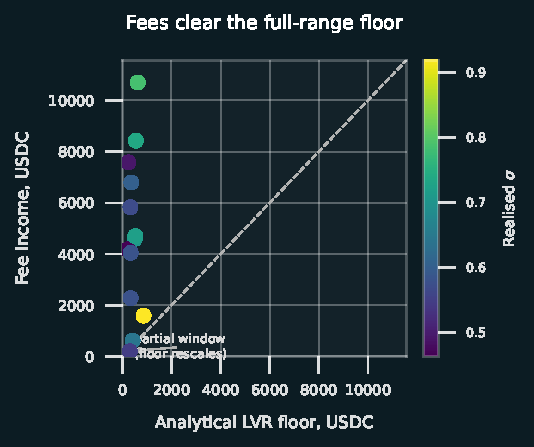
\includegraphics[width=0.62\linewidth]{figures/fee_lvr.pdf}
\caption{Fee income of the opening band against the analytical full-range LVR
floor $0.125\,\sigma^2Vt$, one point per evaluation window, coloured by the
window's realised volatility. The dashed line is where fees exactly cover the
floor. The annotated point is the partial final window, whose floor rescales to
its length.}
\label{fig:fee-lvr}
\end{figure}

\begin{table}[tbp]
\caption{The boundary sweep on the $0.05\,\%$ pool. Values are mean PnL in USDC
over the thirteen evaluation windows, with Sharpe in parentheses. The gas
levels scale the per-action gas cost. The capital levels scale the book. The
last column is the best validation seed of the main run.}
\label{tab:boundary}
\centering
\small
\begin{tabular}{@{}L{0.15\linewidth}rrrrr@{}}
\toprule
\textbf{Level} & \textsf{hodl} & \textsf{wide} & \textsf{tau\_reset} & \textsf{cost\_aware} & best seed \\
\midrule
Gas $\times0.25$ & $+735$ (0.65) & $+1\,651$ (1.53) & $-11\,613$ ($-3.72$) & $-2\,953$ ($-0.54$) & $+203$ (1.42) \\
Gas $\times1$ & $+735$ (0.65) & $+1\,623$ (1.53) & $-17\,680$ ($-5.81$) & $-1\,992$ ($-0.24$) & $+175$ (1.42) \\
Gas $\times4$ & $+735$ (0.65) & $+1\,509$ (1.53) & $-40\,032$ ($-12.85$) & $-1\,419$ (0.01) & $+65$ (1.42) \\
Capital 10k & $+81$ (0.68) & $+128$ (1.53) & $-6\,764$ ($-15.37$) & $-195$ ($-0.10$) & $-13$ (1.46) \\
Capital 100k & $+735$ (0.65) & $+1\,623$ (1.53) & $-17\,680$ ($-5.81$) & $-1\,992$ ($-0.24$) & $+175$ (1.42) \\
Capital 1M & $+1\,384$ (0.46) & $+16\,213$ (1.51) & $-162\,687$ ($-5.47$) & $-54\,962$ ($-1.35$) & $+2\,003$ (1.40) \\
\bottomrule
\end{tabular}
\end{table}

\begin{table}[tbp]
\caption{Mean PnL (top panel) and mean CVaR at $5\,\%$ (bottom panel) in USDC
by dominant regime label over the 2024 evaluation windows. There are five bear
windows, five bull windows, two sideways windows and one high-volatility
window. The Width 50 and Width 202 columns are the narrow ($\pm5\,\%$) and wide
($\pm20\,\%$) one-shot bands, whose mean half-widths are 50 and 202 tick
spacings. The column for the best seed reports the seed with the highest
validation Sharpe on the training split. The single high-volatility window is a
case study, not a distribution.}
\label{tab:regimes}
\centering
\small
\begin{tabular}{@{}L{0.19\linewidth}rrrrrr@{}}
\toprule
 & \multicolumn{6}{c}{\textbf{Mean PnL (USDC)}} \\
\cmidrule(lr){2-7}
\textbf{Regime (windows)} & \textsf{hodl} & Width 50 & Width 202 & Full range & Delta hedge & Best seed \\
\midrule
Bear (5) & $+317$ & $+1\,772$ & $+2\,589$ & $+1\,044$ & $-1\,707$ & $+527$ \\
Bull (5) & $+4\,335$ & $+4\,127$ & $+4\,779$ & $+7\,379$ & $-1\,958$ & $+1\,093$ \\
Sideways (2) & $+4\,648$ & $+3\,558$ & $+1\,693$ & $-550$ & $-3\,145$ & $+74$ \\
High volatility (1) & $-23\,000$ & $-22\,542$ & $-19\,123$ & $-12\,642$ & $-1\,330$ & $-5\,969$ \\
\midrule
 & \multicolumn{6}{c}{\textbf{Mean CVaR at $5\,\%$ (USDC)}} \\
\cmidrule(lr){2-7}
Bear (5) & $-78.3$ & $-74.3$ & $-57.3$ & $-49.2$ & $-2.0$ & $-19.6$ \\
Bull (5) & $-31.9$ & $-31.2$ & $-37.0$ & $-58.3$ & $-4.1$ & $-12.8$ \\
Sideways (2) & $-65.0$ & $-59.3$ & $-50.8$ & $-49.6$ & $-4.4$ & $-15.8$ \\
High volatility (1) & $-94.5$ & $-94.4$ & $-93.9$ & $-54.5$ & $-1.4$ & $-27.8$ \\
\bottomrule
\end{tabular}
\end{table}
